\documentclass{article}
%==============================================================================%
%	                          Packages                                     %
%==============================================================================%
% Packages
\usepackage[utf8]{inputenc}
\usepackage{graphicx}
\usepackage{float}
\usepackage{amsmath}
\usepackage{amssymb}
\usepackage{braket}
\usepackage{subcaption}
\usepackage[margin=0.7in]{geometry}
\usepackage[version=4]{mhchem}
%==============================================================================%
%                           User-Defined Commands                              %
%==============================================================================%
% User-Defined Commands
\newcommand{\be}{\begin{equation}}
\newcommand{\ee}{\end{equation}}
\newcommand{\benum}{\begin{enumerate}}
\newcommand{\eenum}{\end{enumerate}}
\newcommand{\pd}{\partial}
\newcommand{\dg}{\dagger}
\newcommand{\sumzero}{\sum_{n=0}^\infty}
\newcommand{\sumone}{\sum_{n=1}^\infty}
%==============================================================================%
%                             Title Information                                %
%==============================================================================%
\title{Chem237: Lecture 8}
\date{4/10/18}
\author{Alan Robledo}
%==============================================================================%
%	Everyone Please Make Comments if Something Needs to be Reviewed        %
%                           Or just fix it yourself!                           %
%==============================================================================%
\begin{document}
\maketitle

\section*{Approximate Methods}
So far, we have discussed different ways to evaluate integrals of interest to obtain exact answers.
It is often times enough for us to know an approximation to the value of an integral and we will discuss a few methods that go about doing this by looking at some special functions as examples.
\subsection*{Asymptotic Series}
At first glance, you'd think that the error function is just the integral of a gaussian
\be
  \text{erf(x)} = \frac{2}{\sqrt{\pi}} \int_0^x e^{-t^2} dt = \frac{1}{\sqrt{\pi}} \int_{-x}^x e^{-t^2} dt
\ee
and you'd be correct. To be specific, the error function is the integral of a normalized Gaussian with the normalization part coming from the $\frac{1}{\sqrt{\pi}}$.
The error function comes up in probability theory as this function is used to show the probability of something lying between -x and x.
Finding a good approximation of the integral can be done by taylor expanding the integrand about a center that we will take to be zero, and integrating term by term.
\be
  \begin{split}
    \text{erf(x)} &= \frac{2}{\sqrt{\pi}} \int_0^x e^{-t^2} dt \\
    &= \frac{2}{\sqrt{\pi}} \int_0^x (1 - t^2 + \frac{t^4}{2!} - \frac{t^6}{3!} + \hdots) dt \\
    &= \frac{2}{\sqrt{\pi}} (x - \frac{x^3}{3} + \frac{x^5}{5 \cdot 2!} - \frac{x^7}{7 \cdot 3!} + \hdots)
  \end{split}
\ee
By the look of it, we can say that the series converges for any x because the denominator tends to infinity much faster than the numerator ever could.
However, the convergence of the series is small for large x.
As a matter of fact, for large x, as x $\rightarrow \infty$, erf(x) $\rightarrow$ 1.
So suppose we wanted to know what erf(x) is for large x.
Using the fact that erf(x) $\rightarrow$ 1 as x $\rightarrow \infty$, we could write
\be
1 = \frac{2}{\sqrt{\pi}} \int_0^{\infty} e^{-t^2} dt
\ee
and if we break up the integrals
\be
1 = \frac{2}{\sqrt{\pi}} \int_0^x e^{-t^2} dt + \frac{2}{\sqrt{\pi}} \int_x^{\infty} e^{-t^2} dt
\ee
and rearrange terms, we get
\be \label{eq:erfc}
1 - \frac{2}{\sqrt{\pi}} \int_0^x e^{-t^2} dt = 1 - \text{erf(x)} = \frac{2}{\sqrt{\pi}} \int_x^{\infty} e^{-t^2} dt = \text{erfc(x)}
\ee
where we have an integral from large x to infinity, which happens to be called the complementary error function or erfc(x).
We can try to find an expression for the complementary error function by considering using integration by parts.
Now, you may look at the integrand and think to yourself that there are no two functions that you can use for integration by parts.
But a neat little trick that is often used is to consider multiplying the integrand by the one function.
\be
  \int_x^{\infty} e^{-t^2} dt = \int_x^{\infty} e^{-t^2} \cdot 1 dt = \int_x^{\infty} e^{-t^2} \cdot \frac{-2t}{-2t} dt
\ee
and if we consider,
\be
  \begin{split}
    U &= - \frac{1}{2t} \qquad dV = - 2t e^{-t^2} dt \\
    dU &= \frac{1}{2t^2} dt \qquad V = e^{-t^2}
  \end{split}
\ee
our integral becomes
\be
  \begin{split}
    \int_x^{\infty} e^{-t^2} dt &= \frac{e^{-t^2}}{2t} \Big|_x^{\infty} - \int_x^{\infty} \frac{e^{-t^2}}{2t^2} dt \\
    &= \frac{e^{-x^2}}{2x} - \int_x^{\infty} \frac{e^{-t^2}}{2t^2} dt
  \end{split}
\ee
We can integrate by parts again by using the same trick of multiplying the integrand by the one function
\be
  \int_x^{\infty} e^{-t^2} dt = \frac{e^{-x^2}}{2x} - \int_x^{\infty} \frac{e^{-t^2}}{2t^2} \cdot \frac{-2t}{-2t} dt
\ee
and considering
\be
  \begin{split}
    U &= - \frac{1}{4t^3} \qquad dV = - 2t e^{-t^2} dt \\
    dU &= \frac{3}{4t^4} dt \qquad V = e^{-t^2}
  \end{split}
\ee
to get
\be
  \begin{split}
    \int_x^{\infty} e^{-t^2} dt &= \frac{e^{-x^2}}{2x} - \int_x^{\infty} \frac{e^{-t^2}}{2t^2} \\
    &= \frac{e^{-x^2}}{2x} + \frac{e^{-t^2}}{4t^3} \Big|_x^{\infty} + \int_x^{\infty} \frac{3e^{-t^2}}{4t^4} dt \\
    &= \frac{e^{-x^2}}{2x} - \frac{e^{-x^2}}{4x^3} + \int_x^{\infty} \frac{3e^{-t^2}}{4t^4} dt
  \end{split}
\ee
You can see that we can use this trick each time we integrate by parts and if we integrated an infinite number of times, we'd have an exact expression.
If we go back to equation \ref{eq:erfc} and solve for erf(x), we can see that the result after n integrations by parts of the complementary error function gives
\be
  \begin{split}
    \text{erf(x)} = 1 - \frac{2}{\sqrt{\pi}} \int_x^{\infty} e^{-t^2} dt = 1 - \frac{2}{\sqrt{\pi}} e^{-x^2} \Big[ \frac{1}{2x} - \frac{1}{2^2 x^3} & + \frac{1 \cdot 3}{2^3 x^5} - \frac{1 \cdot 3 \cdot 5}{2^4 x^7} + \hdots + (-1)^{n-1} \frac{1 \cdot 3 \cdot 5 \cdots (2n-3)}{2^n x^{2n-1}} \Big] \\
    & + (-1)^n \frac{1 \cdot 3 \cdot 5 \cdots (2n-1)}{2^n} \frac{2}{\sqrt{\pi}} \int_x^{\infty} \frac{e^{-t^2}}{t^{2n}} dt
  \end{split}
\ee
where the last term (the term after the brackets, including the integral) is the "remainder" that makes the expression exact.
If we only pay attention to the terms inside the brackets, we can see that these terms form the beginning of a divergent series.
Since the numerator grows as (2n+1)!, there is no value of x that would make the denominator grow larger in size than the numerator so if we were to form an infinite series from the terms in the brackets, this series would diverge to $\infty$.
It is because of this fact that physicists would call the series in brackets an \textbf{asymptotic series} if the summation of the terms continued to infinity.
To be formal, if we have a function whose series expansion is
\be
S(x) = c_0 + \frac{c_1}{x} + \frac{c_2}{x^2} + \hdots
\ee
where the c$_n$'s are just constants, we can say that the partial sum $\sum\limits_{i=0}^n c_i / x^i$ is an asymptotic series expansion of f(x) if the following holds
\be
  \lim_{x \to \infty} x^n \Big[ f(x) - \sum_{i=0}^n \frac{c_i}{x^i} \Big] = 0
\ee
Therefore, for some value n and for arbitrarily large x, the series $S_n(x)$ gives a good approximation to f(x).
If, however, we have a function whose series expansion is
\be
  S(x) = c_0 + c_1x + c_2x^2 + \hdots
\ee
where the c$_n$'s are again just constants, we can say that the partial sum  $\sum\limits_{i=0}^n c_i x^i$ is an asymptotic series expansion of f(x) if the following holds
\be
  \lim_{x \to \infty} \frac{1}{x^n} \Big[ f(x) - \sum_{i=0}^n c_i x^i \Big] = 0
\ee
Therefore, for some value n and for arbitrarily small x, the series $S_n(x)$ gives a good approximation to f(x).

Mathematicians define an asymptotic series expansion as a series whose partial sums give a good approximation to a function of a variable x for arbitrarily small or large values of x.
This definition makes it sound like a convergent Taylor series falls under the category of an asymptotic expansion.
Because of this, it is common in Physics for the term 'asymptotic expansion' to imply a divergent series.
To be mathematically correct, an asymptotic series can be divergent or convergent but, in most cases of interest, asymptotic series never converge.
So it is useful to consider the physicist's perspective when distinguishing between a convergent series and an asymptotic series.
We can go back to the error function erf(x) to show how an asymptotic series can be different from a convergent series.
\be
  \text{erf(x)} = \frac{2}{\sqrt{\pi}} \int_0^x e^{-t^2} dt
\ee
Just as we did in equation 2, if we taylor expand the integrand about $t=0$, and integrate the series term by term, we get the following convergent series,
\be
  \text{erf(x)} = \frac{2}{\sqrt{\pi}} \Big( x - \frac{1}{3}x^3 + \hdots + \frac{(-1)^n}{(2n+1)n!} x^{2n+1} + \hdots \Big)
\ee
which is convergent for all values of x.
And if we recall from earlier, we obtained an asymptotic series of the erf(x) from continuous integrations by parts
\be
  \text{erf(x)} \approx 1 - \frac{2}{\sqrt{\pi}} e^{-x^2} \Big[ \frac{1}{2x} - \frac{1}{2^2 x^3} + \frac{1 \cdot 3}{2^3 x^5} - \frac{1 \cdot 3 \cdot 5}{2^4 x^7} + \hdots + (-1)^{n-1} \frac{1 \cdot 3 \cdot 5 \cdots (2n-3)}{2^n x^{2n-1}} \Big]
\ee
where the asymptotic series is just the terms in the brackets minus the remainder.
Now, when $x=3$, we need the first 30 terms of the taylor series to approximate erf(3) to an accuracy of $10^{-5}$, whereas we only need the first two terms of the asymptotic series to obtain the same approximation.
This should not be of any surprise to us because I mentioned earlier in the lecture that the convergence of the Taylor series is slow for (arbitrarily) large x.
If we were to make a plot of the remainder as a function of the number of terms we decide to keep in our series approximation for fixed x
%==============================================================================%
%  Add plot of remainder as a function of M in notes.
%==============================================================================%
we would see that as we keep adding more terms, our approximation gets better and better up to a certain limit, which defines the asymptoticity of the function, and then our approximation becomes worse and worse as we add even more terms.
It makes sense that the remainder blows up to infinity because we are trying to use a divergent series to define the value of an integral.

Note, if we use the Physics definition of an asymptotic series then we have to be clear in saying that not all functions have an asymptotic expansion.
If a function does have such an expansion then that expansion is unique.
However, one can get different asymptotic series expansions for the same function if we consider x to be a complex number z and the convergence of a series to be defined by the radius of a disk on the complex plane.
This is known in complex analysis as Stokes phenomenon but we will not dive into the topic.

\subsection*{Saddle Point Method}
To introduce another method of integral approximations, we will consider the integral
\be
  \int_0^{\infty} F(x) dx = \int_0^{\infty} e^{f(x)} dx
\ee
where the integral of F(x) is dominated by a narrow region in x.
A example plot of F(x) as a function of x would be
%==============================================================================%
%  Add plot of generic gaussian.
%==============================================================================%
If we perform a Taylor expansion of f(x) and decide to expand around the point x$_o$ we get
\be
  F(x) \approx \text{exp} \Big[ f(x_o) + (x - x_o)f'(x_o) + \frac{(x - x_o)^2}{2}f''(x_o) \Big]
\ee
If we let x$_o$ to be the maximum of f(x), we can identify that $f'(x_o) = 0$ so our integral becomes
\be
  \begin{split}
    \int_0^{\infty} F(x) dx &\approx \int_0^{\infty} \text{exp} \big[ f(x_o) + \frac{(x - x_o)^2}{2}f''(x_o) \Big] dx \\
    &= \text{exp}[f(x_o)] \int_0^{\infty} \text{exp} \Big[ \frac{(x - x_o)^2}{2}f''(x_o) \Big] dx
  \end{split}
\ee
which is just the integral of a gaussian exp $[A(x-x_o)^2]$ where $A = \frac{f''(x_o)}{2}$.
Using a u-substitution $u = x - x_o$ and $du = dx$, you should be able to get
\be
  \begin{split}
      \int_0^{\infty} F(x) dx &\approx \text{exp}[f(x_o)] \int_0^{\infty} \text{exp} \Big[ \frac{(x - x_o)^2}{2}f''(x_o) \Big] dx \\
      &= \text{exp}[f(x_o)] \Big( \frac{-2 \pi}{f''(x_o)} \Big) ^{\frac{1}{2}}
  \end{split}
\ee
where $f''(x_o) < 0$ to prevent from obtaining imaginary results.
\subsubsection*{Example}
As an example, we will consider another special function: the Gamma function.
\be
  \Gamma(x+1) = \int_0^{\infty} t^{x} e^{-t} dt
\ee
We can turn the integrand into an exponential with the following transformation
\be
  t^{x} e^{-t} = e^{\ln(t^x)} e^{-t} = e^{x \ln(t)} e^{-t} = e^{x \ln(t) - t}
\ee
and use the saddle-point approximation to approximate the value of the integral.
We will consider $f(t) = x \ln(t) - t$ and Taylor expand $f(t)$ up to second order.
So we need to compute some derivatives and evaluate them at the maximum $t_o$.
\be
  \begin{split}
    f(t) \Big|_{t=t_o} &= x \ln(t_o) - t_o \\
    f'(t) \Big|_{t=t_o} &= \frac{x}{t_o} - 1 \\
    f''(t) \Big|_{t=t_o} &= -\frac{x}{t_o^2}
  \end{split}
\ee
Since we know that the value of the first derivative at the maximum is zero, we can use the second equation to solve for zero and we get the relationship $t_o = x$.
Replacing all the $t_o$'s with x, we get the following expansion
\be
  f(t) \approx x \ln(x) - x - \frac{1}{2!} \cdot \frac{1}{x} (t - x)^2
\ee
So our integral becomes
\be
  \begin{split}
    \Gamma(x+1) &= \int_0^{\infty} t^{x} e^{-t} dt \\
    &= \int_0^{\infty} e^{x \ln(x) - x - \frac{1}{2x} (t - x)^2} \\
    &= \int_0^{\infty} e^{x \ln(x) - x} e^{- \frac{1}{2x} (t - x)^2} dt \\
    &= e^{\ln(x^x) - x} \int_0^{\infty} e^{- \frac{1}{2x} (t - x)^2} dt \\
    &= x^x e^{-x} \int_0^{\infty} e^{- \frac{1}{2x} (t - x)^2} dt
  \end{split}
\ee
which is of course another integral of a gaussian.
Using a u-substitution $u = t - x$ and $du = dx$ (remember, x is considered a constant in this integral) we have
\be
  \begin{split}
    \Gamma(x+1) &\approx x^x e^{-x} \int_0^{\infty} e^{- \frac{1}{2x} (t - x)^2} dt \\
    &= x^x e^{-x} \int_0^{\infty} e^{- \frac{1}{2x} u^2} du \\
    &= \sqrt{2 \pi x} x^x e^{-x} \\
    &= \sqrt{2 \pi x} \Big( \frac{x}{e} \Big)^x
  \end{split}
\ee
which is actually the first half of stirling's approximation!
The second half involves showing that $\Gamma(x+1) = x!$, which can be done by using multiple integration by parts, which shouldn't be too bad.
Taking $t^x = U$ and $e^{-t} = dV$, we get
\be
  \begin{split}
    \Gamma(x+1) &= \int_0^{\infty} t^{x} e^{-t} dt \\
    &= - t^x e^{-t} \Big|_0^{\infty} + x \int_0^{\infty} t^{x-1} e^{-t} dt \\
  \end{split}
\ee
and since $- t^x e^{-t} \Big|_0^{\infty}$ goes to zero, we're just left with $\Gamma(x)$.
So we can integrate by parts a few more times until we see a pattern
\be
  \begin{split}
    \Gamma(x+1) &= x \Gamma(x) \\
    &= x \int_0^{\infty} t^{x-1} e^{-t} dt \\
    &= x \Big( -t^{x-1}e^{-t} \Big|_0^{\infty} + (x-1) \int_0^{\infty} t^{x-2} e^{-t} dt \Big) \\
    &= x(x-1) \int_0^{\infty} t^{x-2} e^{-t} dt \\
    &= x(x-1) \Gamma(x-1) \\
    &= \hdots \\
    &= x(x-1) \cdots 2\cdot1 \int_0^{\infty} e^{-t} dt \\
    &= - (x!) e^{-t} \Big|_0^{\infty} \\
    &= -x! (0 - 1)\\
    &= x!
  \end{split}
\ee
And from our result from earlier, we have that for any integer x = n
\be
  \Gamma(n+1) = n! \approx \sqrt{2 \pi n} \Big( \frac{n}{e} \Big)^n
\ee
which is Stirling's approximation!
%==============================================================================%
% Relate it to Stat mech if you want.
%==============================================================================%
And with that, we are done with chapter 3 of the Math Methods book.
\section*{Integral Transforms}
Chapter 4 can be thought of as a continuation of chapter 3 in that we are still going to be looking at integrals and finding ways to solve them.
But, similar to contour integration, we are going to be focusing on how to map our function of interest from one domain onto another domain in order to make our integrals much easier to solve.
Then we would map our solutions back to the original domain to get the appropriate result.
This is done by considering different types of integral transforms that are used depending on the behavior of our function/integrand.
Some include: Fourier Transform, Laplace Transform, Hilbert Transform, etc, but we will only be discussing the first two as they are very commonly used in Physics.
\subsection*{Fourier Series/Transform}
The topic of Fourier Series/Transform is one that is discussed often in Physics classes and some Physical Chemistry classes.
However, the topic is usually introduced through example and you are only required to know how to obtain the series and/or perform the transform and then understand how it can be applied.
Our Math Methods book introduces the topic the same way.
For those of you who have been taught the subject this way or for those who have only heard of it, you might be aware that there are different conventions associated with the Series/Transform.
But, despite the existence of different conventions, each give the same results to the same problems.

The concept of a Fourier Series is made more intuitive when understood in the context of \textbf{Linear Vector Spaces}.
Linear Vector Spaces are discussed heavily in Linear Algebra courses and are thought about constantly in Quantum Mechanics.
We will be covering Linear Algebra later in the course, but if you have not been exposed to Linear Algebra you can refer to Lecture 11 where we discuss it in full detail.
Or you can try following along until you don't understand something and keep going back and forth with both lectures and whatever other material you may be using.
We will start with some background info that is discussed in any textbook and then we will make the connection to Fourier Series and Fourier Transform.

\subsubsection*{Orthonormality}
One of the nice properties of some functions such as sine and cosine is that they are orthogonal on given intervals.
What it means for two functions to be orthogonal is that if we have, for example, $\sin(nx)$ and $\cos(mx)$ and integrate their product over the interval $0 \leq x \leq 2 \pi$ we get
\be \label{eq:sin_cos}
  \int_0^{2\pi} \sin(nx)\cos(mx) dx = 0
\ee
for any integers n and m.
If we have a similar integral but instead with two functions of the same type, such as $\sin(nx)$ and $\sin(mx)$, then we get
\be \label{eq:sin_sin_orth}
\int_0^{2\pi} \sin(nx)\sin(mx) dx =
  \left\{
    \begin{array}{ll}
      0 & \quad \text{if} \quad n \neq m \\
      \pi & \quad \text{if} \quad n = m
    \end{array}
  \right.
\ee
Likewise, if we have two cosine functions $\cos(nx)$ and $\cos(mx)$, then
\be \label{eq:cos_cos_orth}
\int_0^{2\pi} \cos(nx)\cos(mx) dx =
  \left\{
    \begin{array}{ll}
      0 & \quad \text{if} \quad n \neq m \\
      \pi & \quad \text{if} \quad n = m
    \end{array}
  \right.
\ee
where, again, n and m are integers $n,m = 1, 2, 3, \hdots$.
If we wanted to normalize a function, then we must consider our function of interest carrying around a normalization constant $a_n$ such that the integral of the function times itself over some interval is equal to one, i.e. $\int |f(x)|^2 dx = 1$.
If we had complex functions, we would need to be careful with the square modulus $|f(x)|^2$, because the modulus is defined as
\be
  |f(x)|^2 = f^*(x) f(x)
\ee
where $f^*(x)$ denotes the complex conjugate.
If you have a real function, then the square modulus is simply the function times itself.
If we do this for a real function $a_n \sin(nx)$, this would look like
\be \label{eq:sin_sin_norm_norm}
  \int_0^{2\pi} a_n^2 \sin^2(nx) = a_n^2\pi = 1
\ee
and we can use this to find the normalization constant.
\be
  a_n^2\pi = 1 \Rightarrow a_n = \frac{1}{\sqrt{\pi}}
\ee
If we do this for another function $b_n \cos(nx)$, we can find its normalization constant $b_n$
\be \label{eq:cos_cos_norm_norm}
  \int_0^{2\pi} b_n^2 \cos^2(nx) = b_n^2\pi = 1 \quad \Rightarrow \quad b_n = \frac{1}{\sqrt{\pi}}
\ee
So if we have two normalized functions that are orthogonal to each other, we say they are orthonormal.
Therefore, if we rewrite equations \ref{eq:sin_sin_orth} and \ref{eq:cos_cos_orth} we get
\be \label{eq:sin_sin_orthonorm}
  \frac{1}{\pi} \int_0^{2\pi} \sin(nx)\sin(mx) dx = \delta_{nm}
\ee
\be \label{eq:cos_cos_orthonorm}
  \frac{1}{\pi} \int_0^{2\pi} \cos(nx)\cos(mx) dx = \delta_{nm}
\ee
where $\delta_{nm}$ is the kronecker delta and it is shorthand notation for
\be
\delta_{nm} =
  \left\{
    \begin{array}{ll}
      0 & \quad \text{if n} \neq \text{m} \\
      1 & \quad \text{if n = m}
    \end{array}
  \right.
\ee
There are usually two conventions, either choosing to normalize your functions or choosing not to normalize your functions.
We will use the convention of using normalized functions so that our integrals either evaluate to 0 or 1 for simplicity.

\subsubsection*{Dirac Notation}
You're probably comfortable with representing vectors as variables with an arrow over it like $\vec{a}$.
So when we say that when we are taking the inner product of two vectors (you may remember this as the dot product), this looks like $\vec{a} \cdot \vec{b}$.
In Physics, we use a different type of notation that means the same thing which is called dirac notation, aka braket notation.
A vector in this notation can be a ket $\ket{a}$ or a bra $\bra{a}$ but it is usually shown as a ket.
So the inner product of two vectors $\vec{u}$ and $\vec{v}$ in braket notation becomes
\be
  \vec{u} \cdot \vec{v} = \braket{u|v}
\ee
and we can remember thinking about the inner product as a projection of some vector $\vec{u}$ onto another vector $\vec{v}$.
%==============================================================================%
% Flashlight image would go here
%==============================================================================%
If we represented a function $f(x)$ as a ket, it could look like $\ket{f(x)}$ or $\ket{f}$.
The naming of a bra or ket is entirely up to you as long as you remember what it represents.
If we had two functions $\ket{f(x)}$ and $\ket{g(x)}$, then $\braket{f(x)|g(x)}$ is defined as an integral of their product
\be
  \braket{f(x)|g(x)} = \int_{- \infty}^{\infty} f^*(x) g(x) dx
\ee
where the upper and lower limits always have to be specified beforehand.
In this case, we are integrating over all space.
Make sure to remember that, when using dirac notation, our function in the ket needs to be in the form of its complex conjugate when evaluating the integral.
Therefore,
\be
  \braket{g(x)|f(x)} = \int_{- \infty}^{\infty} g^*(x) f(x) dx
\ee
and to make the connection to normalization,
\be
  \braket{f|f} = \int_{- \infty}^{\infty} |f(x)|^2 dx
\ee
You could imagine how this could be done to show two functions being orthogonal to each other.

I said earlier that we define vectors in braket notation as bras or kets and if you're confused about why we could treat functions the same way in this notation, it is because we can think of some functions as vectors in a vector space!
I may switch back and forth with representing vectors with arrows or kets but this is just to enforce the idea that they are the same thing.

\subsubsection*{Linear Vector Space}
Linear vector spaces are defined such that each vector in the space needs to follow certain axioms in order for it to be considered a linear vector space.
One property of a vector space that is important to remember is that any vector $\ket{v}$ can be represented as a linear combination of basis vectors $\ket{e_i}$
\be
  \ket{v} = \sum_{i = 0}^{n} a_i \ket{e_i}
\ee
So if we had two basis vectors $\vec{e}_1$ and $\vec{e}_2$, any vector $\vec{v}$ could be represented as
\be
  \ket{v} = a_1 \ket{e_1} + a_2 \ket{e_2}
\ee
where $a_1$ and $a_2$ are coefficients or "weightings" that define how much their repsective basis contributes to the definition of the vector $\vec{v}$.
In terms of functions, a set of infinite polynomials \{$x^0, x^1, x^2, x^3, \hdots$\} can be considered a basis in a vector space where every vector is itself a polynomial (this is first thing that is proven in every standard Linear Algebra course but we will not prove it here so take my word for it).
So any polynomial can be represented as
\be
  \ket{v} = \sum_{i=1}^{n} a_i \ket{e_i} = \sum_{i=1}^{n} a_i x^i
\ee
where n defines the dimensions of the space.
So if we have an infinite number of basis vectors, we have an infinite dimensional space.

Remember that whenever we have a function, we can almost always represent it in a Taylor series expansion, giving us
\be
  f(x) = \sum_{n=0}^{\infty} a_n x^n
\ee
where $a_n$ is defined as
\be
  a_n = \frac{f^{(n)}(x_o)}{n!}
\ee
If you haven't noticed yet where I'm going with this, we could think of our expanded function $f(x)$ as a vector that is represented as a linear combination of basis vectors \{$x^0, x^1, x^2, x^3, \hdots$\}.

Now that we have a vector space, we want to be able to define an inner product on our space.
The reason why we want to define an inner product is because we want to be able to define an orthogonal projection of one vector onto another, as I've explained before.
When we project a vector $\vec{u}$ onto another vector $\vec{v}$, we consider this as taking the dot product
\be
  \vec{u} \cdot \vec{v} = u_1v_1 + u_2v_2 + \hdots
\ee
And since our functions can be thought of as vectors, we can think of performing an inner product with our functions because taking an integral is exactly the same thing as the inner product!

When we have two vectors, the dot product is defined as multiplying a component from one vector and a component from another vector and adding up all the multiplications.
When we have two functions f and g, the integral of their product is defined as multiplying a function evaluated at a point and another function evaluated at a point, with each product having a weight dx, and adding up all the multiplications.
\be
  \int_a^b f(x)g(x) = f(a)g(a)dx + f(a + dx)g(a + dx)dx + \hdots
\ee
So our inner product for functions is the same thing as taking the integral of the product of our functions!
\be
  \braket{f|g} = \int_a^b f^*(x)g(x) dx
\ee

\subsection*{Fourier Series}
In lecture 3, we showed that sine and cosine both have Taylor expansions of the form
\be
  \begin{split}
    \sin(x) &= x - \frac{x^3}{3!} + \frac{x^5}{5!} - \hdots \\
    \cos(x) &= 1 - \frac{x^2}{2!} + \frac{x^4}{4!} - \hdots
  \end{split}
\ee
where $\sin(x)$ and $\cos(x)$ are functions of x with odd and even powers, respectively.
If we add $\sin(x)$ and $\cos(x)$ together, we get an infinite degree polynomial in x.
\be
  \cos(x) + \sin(x) = (1 - \frac{x^2}{2!} + \frac{x^4}{4!} - \hdots) + (x - \frac{x^3}{3!} + \frac{x^5}{5!} - \hdots) = 1 + x - \frac{x^2}{2!} - \frac{x^3}{3!} + \frac{x^4}{4!} + \hdots
\ee
Therefore, we can think of $\cos(nx)$ and $\sin(nx)$, where n is an integer, as being basis vectors in a space where every vector is written as a linear combination of them
\be
  \ket{f} = \sum_{n = 0}^{\infty} A_n \ket{\cos(nx)} + B_n \ket{\sin(nx)}
\ee
And if we don't use dirac notation for a second and replace x with $\theta$, we recover the exact form of a Fourier series!
\be
  f(\theta) = \sum_{n = 0}^{\infty} A_n \cos(n \theta) + B_n \sin(n \theta)
\ee
So every time we see a Fourier series, we can think of it as just a vector $f(\theta)$ that is represented as a linear combination of basis vectors $\cos(n \theta)$ and $\sin(n \theta)$.
And we will see that we can easily find an expression for the coefficients through the use of dirac notation.
If you're thinking ahead, we can also have a complex exponential $e^{ix}$ or $e^{-ix}$ as a basis vector as well, but we will consider this later in lecture.

While we are able to think of a series as a sum of vectors, a Fourier series can only be created from functions $f(\theta)$ that are defined periodically for intervals of length L.
When we say that a function is periodic, we mean that the function repeats in intervals, e.g. $- 2\pi \leq \theta \leq 0$, $- \pi \leq \theta \leq \pi$, $2 \pi \leq \theta \leq 4 \pi $, etc.
It is only required that the interval is of a certain length, in this case $2 \pi$.
For the time being, we will stick to the interval $0 \leq \theta \leq 2 \pi$ and discuss changing the length later because the length of the interval does not change how we find the coefficients.

We will be using the convention of having our basis vectors be normalized so that our Fourier series is now
\be
  \ket{f(\theta)} = \sum_{n=0}^{\infty} A_n \ket{c_n} + B_n \ket{s_n}
\ee
where $\ket{c_n} = \frac{1}{\sqrt{\pi}} \cos(n \theta)$ and $\ket{s_n} = \frac{1}{\sqrt{\pi}} \sin(n \theta)$, where $\frac{1}{\sqrt{\pi}}$ is the normalization constant we derived earlier in lecture.
Now that we know how to take dot products in braket notation, we can use our functions' orthogonality properties to find an expression for the coefficients $A_n$ and $B_n$.

If we wanted to find the n-th term of a Fourier series, we can consider projecting the cosine vector $\bra{c_n}$ onto the n-th term of our $\ket{f(\theta)}$ vector (remember, projection means dot product) and we get,
\be
  \braket{c_n|f(\theta)} = \bra{c_n} \Big( A_n \ket{c_n} + B_n \ket{s_n} \Big) = A_n \braket{c_n|c_n} + B_n \braket{c_n|s_n}
\ee
and since we know from equation \ref{eq:sin_cos} that the integral of sine and cosine is always zero, then the dot product $\braket{c_n|s_n}$ is always zero.
And since we know from equation \ref{eq:cos_cos_orthonorm} that $\braket{c_n|c_n}$ is 1 when $n = m$, then all we're left with is
\be
  A_n = \braket{c_n|f(\theta)} = \frac{1}{\sqrt{\pi}} \int_0^{2\pi} \cos(n \theta) f(\theta) d\theta
\ee
If we project the sine vector $\bra{s_n}$ onto the n-th term of our $\ket{f(\theta)}$ vector, we get,
\be
  \braket{s_n|f(\theta)} = \bra{s_n} \Big( A_n \ket{c_n} + B_n \ket{s_n} \Big) = A_n \braket{s_n|c_n} + B_n \braket{s_n|s_n}
\ee
And using the same logic as before, equation \ref{eq:sin_cos} says that $\braket{s_n|c_n}$ is zero for any n and m, and equation \ref{eq:sin_sin_orthonorm} says $\braket{s_n|s_n}$ will only be 1 when $n = m$, so we're left with
\be
  B_n = \braket{s_n|f(\theta)} = \frac{1}{\sqrt{\pi}} \int_0^{2\pi} \sin(n \theta) f(\theta) d\theta
\ee
If you check to see what our Math methods book has for the coefficients $A_n$ and $B_n$, you'll notice that there is a factor of $\frac{1}{\pi}$ in front of the integrals, whereas we have $\frac{1}{\sqrt{\pi}}$.
The reason for this is because (and some books do not mention this explicitly like ours) the book is choosing the convention where the basis functions are not normalized, whereas we have chosen to use the convention where the basis functions are normalized.
If you're starting to think that our convention is wrong, watch what happens when we explicitly write the fourier series with the coefficients written in their integral form using our convention.
\be \label{eq:fourier_check}
  \begin{split}
    f(\theta) &= \sum_{n = 0}^{\infty} \Big( \frac{1}{\sqrt{\pi}} \int_0^{2\pi} \cos(n \theta) f(\theta) d\theta \Big) \frac{1}{\sqrt{\pi}} \cos(n \theta) + \Big( \frac{1}{\sqrt{\pi}} \int_0^{2\pi} \sin(n \theta) f(\theta) d\theta \Big) \frac{1}{\sqrt{\pi}} \sin(n \theta) \\
    &= \sum_{n = 0}^{\infty} \Big( \frac{1}{\pi} \int_0^{2\pi} \cos(n \theta) f(\theta) d\theta \Big) \cos(n \theta) + \Big( \frac{1}{\pi} \int_0^{2\pi} \sin(n \theta) f(\theta) d\theta \Big) \sin(n \theta)
  \end{split}
\ee
The Fourier series coefficients end up becoming exactly as the book has them written.
So both conventions give the same result.
An issue that occurs in scientific computing is that some math software packages will program Fourier series such that there are no $\sqrt{\pi}$'s or $\pi$'s at all and you are free to add them wherever you like.
This becomes a third convention that simply does not make any sense mathematically and can cause confusion if you come across these packages.
But, now that we know Fourier series are just vectors in a linear vector space with sine and cosine as orthonormal basis vectors, we can use this knowledge as a check to make sure that our math always adds up correctly when we create the series from periodic functions.

This whole time, we've defined our Fourier series in an interval of length $2 \pi$ and we would now like to define a Fourier series that is periodic in an interval of any length L.
So if we wanted our Fourier series to go from representing functions that are periodic with some period $2\pi$ in the variable $\theta$ to representing functions that are periodic with some period L in the variable x, we let
\be
  x = \frac{\theta L}{2 \pi}
\ee
where $\frac{L}{2 \pi}$ can be thought of as a contraction/expansion ratio that is multiplied by our length $\theta$ to get our new length x.
If we rearrange the equation above we get
\be
 \theta = \frac{2 \pi x}{L}
\ee
and our Fourier series is now
\be
 f(\theta) = \sum_{n = 0}^{\infty} A_n \frac{1}{\sqrt{\pi}} \cos \Big( \frac{2 \pi n x}{L} \Big) + B_n \frac{1}{\sqrt{\pi}} \sin \Big( \frac{2 \pi n x}{L} \Big)
\ee
As for our coefficients, we don't need to change the $\frac{1}{\sqrt{\pi}}$ because that comes naturally from our normalized basis.
But we need to make the substitution
\be
  \theta = \frac{2 \pi x}{L} \qquad d\theta = \frac{2 \pi}{L} dx
\ee
into our integrals.
So $A_n$ becomes
\be
  \begin{split}
    A_n &= \braket{c_n|f(x)} \\
    &= \frac{1}{\sqrt{\pi}} \int_0^{L} \cos \Big( \frac{2 n \pi x}{L} \Big) f(x) \frac{2 \pi}{L} dx \\
    &= \frac{1}{\sqrt{\pi}} \frac{2 \pi}{L} \int_0^{L} \cos \Big( \frac{2 n \pi x}{L} \Big) f(x) dx \\
    &= \frac{2 \sqrt{\pi}}{L} \int_0^{L} \cos \Big( \frac{2 n \pi x}{L} \Big) f(x) dx \\
  \end{split}
\ee
and $B_n$ becomes
\be
  \begin{split}
    B_n &= \braket{s_n|f(x)} \\
    &= \frac{2 \sqrt{\pi}}{L} \int_0^{L} \sin \Big( \frac{2 n \pi x}{L} \Big) f(x) dx \\
  \end{split}
\ee
which is now defined on an interval of length L such as $0 \leq x \leq L$, $-L \leq x \leq 0$, etc.
Again, the book defines the coefficients with a $\frac{2}{L}$ but I can assure you that if you plug in our coefficients like I did in equation \ref{eq:fourier_check}, both conventions will yield the same series.

Now that we have a full understanding of where a Fourier series comes from, we will see how much easier it will be to define Fourier Transforms using our convention.
But for now, we will consider some examples that require us to create a Fourier Series to see where it can be applied.
However, we basically covered how to create a Fourier series if we are given any periodic function $f(\theta)$ or $f(x)$.
Therefore, we will consider some special cases where our given function is a periodic even or odd function.

If we have a periodic odd function, we say that $-f(\theta) = f(-\theta)$.
And if we wanted to represent an odd function as a Fourier series, we could use the fact that sine is an odd function and cosine is an even function to deduce that we will not have any cosine contribution.
This means that we can skip having to evaluate the $A_n$ coefficients because $A_n$'s dictate the amount of cosine contribution, which we concluded is always zero.
And all we need to evaluate are the $B_n$'s and we would be done.

If we have a periodic even function, we say that $f(\theta) = f(- \theta)$.
And using the same logic as before, we can skip having to evaluate the $B_n$ coefficients because $B_n$'s dictate the amount of sine contribution, which we can conclude is always zero.
So all we would need to evaluate are the $A_n$'s and we would be done.

\subsubsection*{Example}
As our first example, consider the following plot of $f(\theta)$
\begin{figure}[H]
  \centering
  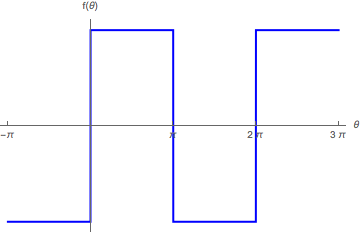
\includegraphics[scale=0.7]{figures/SquareWave.png}
    \caption{Plot of the square wave function from $- \pi \leq \theta \leq 3 \pi$.}
\end{figure}
where the function can be defined as a piecewise function.
\be
  f(x) =
  \left\{
    \begin{array}{ll}
      +1 & \quad 0 < \theta < \pi \\
      -1 & \quad \pi < \theta < 2 \pi
    \end{array}
  \right.
\ee
If we make a plot of the piecewise function from $- \pi$ to $\pi$ with a plot of $\sin(x)$ superimposed on top of it,
\begin{figure}[H]
  \centering
  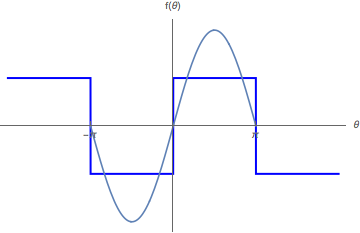
\includegraphics[scale=0.7]{figures/square_sin_plot.png}
    \caption{A sine wave from $- \pi \leq \theta \leq \pi$ superimposed on the square wave. Notice that one sine function $\sin(x)$ already shows similar behavior to the square wave function.}
\end{figure}
we can see that this function is an odd function, so we will only need $B_n$'s when creating a Fourier series representation.
Since $\sin(n \theta) = 0$ when $n = 0$, we don't have to consider the $B_0$ term and only consider $n = 1, 2, 3, \hdots$.
We then have
\be
  B_n = \braket{s_n|f(\theta)} = \frac{1}{\sqrt{\pi}} \int_0^{2 \pi} sin(n \theta) f(\theta) d\theta
\ee
where our upper and lower limits come from noticing that our function is periodic from 0 to $2 \pi$.
Since our function has different forms in the intervals $0 < \theta < \pi$ and $\pi < \theta < 2 \pi$, we could split up our integral into two integrals and evaluate
\be
  \begin{split}
    B_n &= \braket{s_n|f(\theta)} \\
    &= \frac{1}{\sqrt{\pi}} \int_0^{2 \pi} \sin(n \theta) f(\theta) d\theta \\
    &= \frac{1}{\sqrt{\pi}} \int_0^{\pi} \sin(n \theta) \cdot 1 d\theta + \frac{1}{\sqrt{\pi}} \int_{\pi}^{2 \pi} \sin(n \theta) \cdot -1 d\theta \\
    &= \frac{1}{\sqrt{\pi}} \Big( - \frac{\cos(n \theta)}{n} \Big) \Big|_0^{\pi} + \frac{1}{\sqrt{\pi}} \Big( \frac{\cos(n \theta)}{n} \Big) \Big|_{\pi}^{2 \pi} \\
    &= \Big( - \frac{\cos(n \pi)}{n \sqrt{\pi}} + \frac{1}{n \sqrt{\pi}} \Big) + \Big( \frac{\cos(2 n \pi)}{n \sqrt{\pi}} - \frac{\cos(n \pi)}{n \sqrt{\pi}} \Big)
  \end{split}
\ee
Since $n = 1, 2, 3, \hdots$, we can say that $\cos(2 n \pi)$ will always be equal to 1, because any value of n will give this result.
\be
  \begin{split}
    B_n &= \frac{1}{\sqrt{\pi}} \int_0^{2 \pi} \sin(n \theta) f(\theta) d\theta \\
    &= \Big( - \frac{\cos(n \pi)}{n \sqrt{\pi}} + \frac{1}{n \sqrt{\pi}} \Big) + \Big( \frac{1}{n \sqrt{\pi}} - \frac{\cos(n \pi)}{n \sqrt{\pi}} \Big) \\
    &= \frac{-2 \cos(n \pi)}{n \sqrt{\pi}} + \frac{1}{n \sqrt{\pi}} + \frac{1}{n \sqrt{\pi}} \\
    &= \frac{-2 \cos(n \pi)}{n \sqrt{\pi}} + \frac{2}{n \sqrt{\pi}}
  \end{split}
\ee
We cannot say that $\cos(n \pi)$ will always be equal to 1 because it can alternate in sign.
But, we since we know that it will either be 1 or $-1$ depending on the value of n, we can replace $\cos(n \pi)$ with $(-1)^n$, giving
\be
  \begin{split}
    B_n = \frac{-2 (-1)^n}{n \sqrt{\pi}} + \frac{2}{n \sqrt{\pi}} = \frac{2 (-1)^{n+1}}{n \sqrt{\pi}} + \frac{2}{n \sqrt{\pi}} = \frac{2}{n \sqrt{\pi}} ((-1)^{n+1} + 1)
  \end{split}
\ee
And this is fine as an answer as long as it is specified that $n = 1, 2, 3, \hdots$.
If you wanted to make this answer cleaner, you can say that
\be
  B_n =
  \left\{
    \begin{array}{ll}
      0 & \quad \text{for all even n} \\
      \frac{4}{n \sqrt{\pi}} & \quad \text{for all odd n}
    \end{array}
  \right.
\ee
So our Fourier series becomes
\be
  \begin{split}
    \ket{f(\theta)} &= \sum_{n=0}^{\infty} B_n \ket{s_n} \\
    &=  \sum_{n=1}^{\infty} \Big( \frac{4}{n \sqrt{\pi}} \Big) \frac{1}{\sqrt{\pi}} \sin(n \theta) \\
    f(\theta) &= \frac{4}{\pi} \sum_{n=1}^{\infty} \frac{\sin(n \theta)}{n} \\
    &= \frac{4}{\pi} \Big( \sin(\theta) + \frac{\sin(3 \theta)}{3} + \frac{\sin(5 \theta)}{5} + \hdots \Big)
  \end{split}
\ee
where $n = 1, 3, 5, \hdots$.

If we plot truncated versions of our Fourier series on top of our original function
\begin{figure}[h]
  \centering
  \begin{subfigure}[b]{0.4\textwidth}
    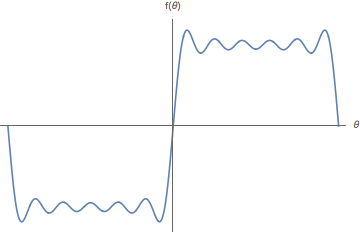
\includegraphics[width=\textwidth]{figures/Sin_0_to_5.png}
    \caption{Plot of the first 6 terms of the Fourier series from $- \pi \leq \theta \leq \pi$.}
  \end{subfigure}
  \hspace{1cm}
  \begin{subfigure}[b]{0.4\textwidth}
    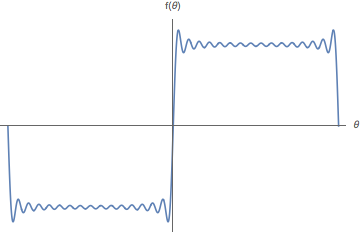
\includegraphics[width=\textwidth]{figures/Sin_0_to_15.png}
    \caption{Plot of the first 16 terms of the Fourier series from $- \pi \leq \theta \leq \pi$.}
  \end{subfigure}
\end{figure}
we can see that if we add more terms from the Fourier series, the series becomes a better and better representation of the original function.
If we notice, the Fourier series function has a peculiar behavior at what is called the "jump discontinuity", where the n-th partial sum shows a maximum (which is called the "overshoot") that is greater than the maximum of the original piecewise function.
And as n approaches infinity, the overshoot does not go to zero but it approaches a finite limit.
This kind of behavior from Fourier series at jump discontinuitiies such as this one is known as Gibb's Phenomenon or Gibb's oscillations.

\subsubsection*{Example}
Consider another example
\be
  f(\theta) = \cos(k \theta) \qquad (- \pi < \theta < \pi)
\ee
where k is any real number so it is not restricted to integers.
Just by looking at the equation, we can immediately tell that we only need cosine terms, so we will only compute the $A_n$'s for $n = 0, 1, 2, \hdots$
\be
  \begin{split}
    A_n &= \braket{c_n|f(\theta)} \\
    &= \frac{1}{\sqrt{\pi}} \int_{-\pi}^{\pi} \cos(n \theta) f(\theta) d\theta \\
    &= \frac{1}{\sqrt{\pi}} \int_{-\pi}^{\pi} \cos(n \theta) \cos(k \theta) d\theta
  \end{split}
\ee
We can exploit the properties of even functions, since an even function times an even function is another even function, and write our integral as
\be
  \frac{1}{\sqrt{\pi}} \int_{-\pi}^{\pi} \cos(n \theta) \cos(k \theta) d\theta
  = \frac{2}{\sqrt{\pi}} \int_{0}^{\pi} \cos(n \theta) \cos(k \theta) d\theta
\ee
And we can substitute a product identity $\cos(x)\cos(y) = \frac{1}{2}[\cos(x - y) + \cos(x + y)]$ to make the integral easier to compute
\be
  \begin{split}
    \frac{2}{\sqrt{\pi}} \int_{0}^{\pi} \cos(n \theta) \cos(k \theta) d\theta &= \frac{2}{\sqrt{\pi}} \int_{0}^{\pi} \frac{1}{2} [\cos(n \theta - k \theta) + \cos(n \theta + k \theta) ] d \theta \\
    &= \frac{1}{\sqrt{\pi}} \int_{0}^{\pi} \cos[(n - k) \theta] d \theta + \frac{1}{\sqrt{\pi}} \int_{0}^{\pi} \cos[(n + k) \theta] d \theta \\
    &= \frac{1}{\sqrt{\pi}} \Big( \frac{\sin[(n - k) \theta]}{(n - k)} \Big) \Big|_0^{\pi} + \frac{1}{\sqrt{\pi}} \Big( \frac{\sin[(n + k) \theta]}{(n + k)} \Big) \Big|_0^{\pi} \\
    &= \frac{1}{\sqrt{\pi}} \frac{\sin[(n - k) \pi]}{(n-k)} + \frac{1}{\sqrt{\pi}} \frac{\sin[(n + k) \pi]}{(n+k)} \\
    &= \frac{1}{\sqrt{\pi}} \frac{(n+k)}{(n+k)} \frac{\sin[(n - k) \pi]}{(n-k)} + \frac{1}{\sqrt{\pi}} \frac{(n-k)}{(n-k)} \frac{\sin[(n + k) \pi]}{(n+k)} \\
    &= \frac{(n+k)}{\sqrt{\pi}} \frac{\sin[(n - k) \pi]}{(n^2-k^2)} + \frac{(n-k)}{\sqrt{\pi}} \frac{\sin[(n + k) \pi]}{(n^2-k^2)} \\
    &= \frac{(n+k)\sin[n \pi - k \pi] + (n-k) \sin[n \pi + k \pi]}{\sqrt{\pi} (n^2 - k^2)} \\
    &= \frac{1}{\sqrt{\pi}(n^2 - k^2)} [(n+k)\sin(n \pi - k \pi) + (n-k) \sin(n \pi + k \pi) ]
  \end{split}
\ee
Using the angle-sum and angle-difference identities $$\sin(x - y) = \sin(x) \cos(y) - \cos(x) \sin(y) \quad \text{and} \quad \sin(x + y) = \sin(x) \cos(y) + \cos(x) \sin(y)$$
we can make another substitution to get
\be
  \begin{split}
    \frac{2}{\sqrt{\pi}} \int_{0}^{\pi} \cos(n \theta) \cos(k \theta) d\theta &= \frac{1}{(n^2 - k^2)} [(n+k)\sin(n \pi - k \pi) + (n-k) \sin(n \pi + k \pi) ] \\
    &= \frac{1}{\sqrt{\pi}(n^2 - k^2)} \Big[ (n+k)[\sin(n \pi)\cos(k \pi) - \cos(n \pi) \sin(k \pi)] + \\
    & \qquad (n - k)[\sin(n \pi)\cos(k \pi) + \cos(n \pi) \sin(k \pi)] \Big]
  \end{split}
\ee
And we can set the two $\sin(n \pi)$'s to zero because n is an integer and we get
\be
  \begin{split}
    \frac{2}{\sqrt{\pi}} \int_{0}^{\pi} \cos(n \theta) \cos(k \theta) d\theta &= \frac{1}{\sqrt{\pi}(n^2 - k^2)} \Big[-(n+k)\cos(n \pi) \sin(k \pi) + (n-k) \cos(n \pi) \sin(k \pi) \Big] \\
    &= \frac{\cos(n \pi) \sin(k \pi)}{\sqrt{\pi}(n^2 - k^2)}[(n-k)-(n+k)] \\
    &= \frac{-2k \cos(n \pi) \sin(k \pi)}{\sqrt{\pi}(n^2 - k^2)} \\
    &= \frac{2k \cos(n \pi) \sin(k \pi)}{\sqrt{\pi}(k^2 - n^2)}
  \end{split}
\ee
which is valid for $n = 0, 1, 2, \hdots$.
If we want to make the result look cleaner, we can do what we did before with $\cos(n \pi)$ and replace it with $(-1)^n$, which gives
\be
  A_n = \frac{2}{\sqrt{\pi}} \int_{0}^{\pi} \cos(n \theta) \cos(k \theta) d\theta = \frac{(-1)^n 2k \sin(k \pi)}{\sqrt{\pi}(k^2 - n^2)}
\ee
So our Fourier series becomes
\be
  \begin{split}
    \ket{f(\theta)} &= \sum_{n=0}^{\infty} A_n \ket{c_n} \\
    &= \sum_{n=0}^{\infty} \Big( \frac{(-1)^n 2k \sin(k \pi)}{\sqrt{\pi}(k^2 - n^2)} \Big) \frac{1}{\sqrt{\pi}} \cos(n \theta) \\
    \cos(k \theta) &= \sum_{n=0}^{\infty} \Big( \frac{(-1)^n 2k \sin(k \pi)}{\pi(k^2 - n^2)} \Big) \cos(n \theta) \\
    &= \frac{2k \sin(k \pi)}{\pi} \sum_{n=0}^{\infty} \frac{(-1)^n \cos(n \theta)}{k^2 - n^2} \\
    &= \frac{2k \sin(k \pi)}{\pi} \Big( \frac{1}{k^2} - \frac{\cos(\theta)}{k^2 - 1} + \frac{\cos(2 \theta)}{k^2 - 4} - \hdots \Big)
  \end{split}
\ee

We've talked about functions where $f(\theta)$ is real so our Fourier series can consist of sines and cosines.
But what if $f(\theta)$ was complex?
All we need to do is change our basis from $\sin(n \theta)$ and $\cos(n \theta)$ to $e^{i n \theta}$.
So we can define our series as
\be
  \ket{f(\theta)} = \sum_{n= - \infty}^{\infty} C_n \ket{e_n}
\ee
where the series goes from $- \infty$ to $\infty$ to cover all space.
We can normalize our basis by requiring that the projection of the basis vector with itself is equal to one $\braket{e_n|e_n} = 1$, which is the same as integrating over our finite interval $0 \leq \theta \leq 2 \pi$.
\be
  \braket{e_n | e_n} = \int_{0}^{2 \pi} c_n^2 e^{-i n \theta} e^{i n \theta} d \theta = c_n^2 \int_{0}^{2 \pi} 1 d \theta = 2 \pi c_n^2 = 1 \quad \Rightarrow \quad c_n = \frac{1}{\sqrt{2 \pi}}
\ee
And we can check that our basis vector is orthogonal with itself by checking if $\braket{e_m|e_n} = 0$.
\be
  \braket{e_m|e_n} = \int_0^{2 \pi} e^{- i m \theta} e^{i n \theta} d \theta = \int_0^{2 \pi} e^{i (n - m) \theta} d\theta = \frac{e^{i (n - m) \theta}}{i (n - m)} \Big|_0^{2 \pi} = \frac{e^{2 i (n - m) \pi}}{i (n - m)} - \frac{e^{0}}{i (n - m)} = \frac{(e^{ i (n - m) \pi})^2}{i (n - m)} - \frac{e^{0}}{i (n - m)}
\ee
Since n and m are integers, then $(n-m)$ is also an integer, and from complex calculus, we know that $e^{i n \pi}$ will either be $+1$ or $-1$ depending on the integer n.
But since $e^{ i (n - m) \pi}$ is squared in our case, it will always be $+1$, so
\be
  \braket{e_m|e_n} = \frac{(e^{ i (n - m) \pi})^2}{i (n - m)} - \frac{e^{0}}{i (n - m)} = \frac{1}{i (n - m)} - \frac{1}{i (n - m)} = 0
\ee
Which means our basis $\ket{e_n}$ is orthonormal and our Fourier series becomes
\be
  \begin{split}
    \ket{f(\theta)} = \sum_{n= - \infty}^{\infty} C_n \ket{e_n} \\
    f(\theta) = \sum_{n= - \infty}^{\infty} C_n \Big( \frac{1}{\sqrt{2 \pi}} e^{i n \theta} \Big)
  \end{split}
\ee
So we can now find an analytic expression for the weight $C_n$ by projecting the basis vector $\ket{e_n}$ onto the n-th term of our function $\ket{f(\theta)}$
\be
  \braket{e_n|f(\theta)} = C_n \braket{e_n|e_n} \quad \Rightarrow \quad C_n = \braket{e_n|f(\theta)} = \frac{1}{\sqrt{2 \pi}} \int_0^{2 \pi} e^{-i n \theta} f(\theta) d \theta
\ee

If we wanted to write a Fourier series for a function that is periodic over a length L, then we substitute $\theta = \frac{2 \pi x}{L}$ and $d\theta = \frac{2 \pi}{L} dx$ to get a new coefficient $C_n$.
\be
  \begin{split}
    C_n = \braket{e_n|f(x)} &= \frac{1}{\sqrt{2 \pi}} \int_0^L e^{- 2 \pi n i / L} f(x) \frac{2 \pi}{L} dx \\
    &= \frac{2 \pi}{L \sqrt{2 \pi}} \int_0^L e^{- 2 \pi n i / L} f(x) dx \\
    &= \frac{\sqrt{2 \pi}}{L} \int_0^L e^{- 2 \pi n i / L} f(x) dx \\
  \end{split}
\ee
Therefore, for any periodic function defined on an interval of length L,
\be
  \ket{f(x)} = \sum_{n = -\infty}^{\infty} C_n \ket{e_n} \Rightarrow f(x) = \sum_{n = -\infty}^{\infty} C_n \frac{1}{\sqrt{2 \pi}} e^{2 \pi n i / L} \qquad C_n = \braket{e_n|f(x)} = \frac{\sqrt{2 \pi}}{L} \int_0^L e^{- 2 \pi n i / L} f(x) dx
\ee

\subsection*{Fourier Transform}
Using everything we used to understand how to obtain a Fourier Series, we will see that performing a Fourier Transform is almost no different.
We've seen that a Fourier Series representation of a function on a finite interval is just a sum over all integers n
\be
  \ket{f(x)} = \sum_{n=-\infty}^{\infty} C_n \ket{e_n}
\ee
where $\ket{e_n}$ is our normalized basis vector $\frac{1}{\sqrt{2 \pi}} e^{ikx}$.
Similarly, a Fourier Transform is just an integral over all real numbers k
\be \label{eq:fourier_trans}
  \ket{f(x)} = f(x) = \frac{1}{\sqrt{2 \pi}} \int_{- \infty}^{\infty} f(k) e^{i k x} dk
\ee
where $f(k)$ can be thought of as our coefficients $C_k$ and $\frac{1}{\sqrt{2 \pi}} e^{ikx}$ can be thought of as our basis vector $\ket{e_n}$.
So, just like in the Fourier Series section, if we wanted to find the k-th coefficient $f(k)$, we just need to project the basis vector onto the function.
\be \label{eq:inverse_fourier}
  \braket{e_n|f(x)} = f(k) = \frac{1}{\sqrt{2 \pi}} \int_{- \infty}^{\infty} e^{-ikx} f(x) dx
\ee
And just like that, we defined the Fourier Transform (equation \ref{eq:fourier_trans}) and the Inverse Fourier Transform (equation \ref{eq:inverse_fourier}).

Notice that the only difference between a Fourier Series and a Fourier Transform is that when we discuss Fourier Series we consider representing functions on a finite interval as a sum of basis vectors with coefficients that are discrete, whereas with Fourier Transforms we consider representing functions on an infinite interval as a sum of basis vectors with coefficients that are continuous.

\end{document}
